
\section{Étude de l'amplitude du déplacement de l'actionneur pour conserver un mouvement naturel} % II 
%\section{Objectif}
\begin{obj}
Déterminer la course des actionneurs permettant de suivre les mouvements du corps conformément à l'exigence Id2 du cahier des charges partiel.
\end{obj}

\ifprof
\else


L'exigence Id2 «~Préserver l'activité musculaire~» est composée de deux exigences Id2.1 et Id2.2 (tableau \ref{ccs_mp_2023_tab_02}). Le fonctionnement de l'exosquelette nécessite une mise en précontrainte. Pour cette mise en précontrainte, chaque actionneur linéaire doit exercer une force de \SI{40}{N}. Cette valeur est obtenue par déplacement vertical de la ceinture haute par rapport à la ceinture basse.

\begin{table}[h]
\begin{center}
\begin{tabular}{lp{5cm}p{5cm}p{2.5cm}l}
\hline
Id & Exigence & Critère & Niveau & Flexibilité \\
\hline
Id2.1 & Permettre le mouvement de translation de la ceinture haute par rapport à la ceinture basse & Déplacement vertical $\Delta h$ de la ceinture haute par rapport à la ceinture basse & $\Delta h=50 \mathrm{~mm}$ & < 10 \% \\
\hline
Id2.2 & Permettre le mouvement de rotation de la ceinture haute par rapport à la ceinture basse & Amplitude de rotation $\varphi$ &  $[0,+20^{\circ}]$  selon l'axe sagittal & < 10 \% \\
\hline
\end{tabular}
%\captionsetup{labelformat=empty}
\caption{\label{ccs_mp_2023_tab_02}Extrait du cahier des charges fonctionnel limité au mouvement dans le plan sagittal de l'exosquelette}
\end{center}
\end{table}
\fi

\subsection{Analyse des exigences 2.1 et 2.2} % Ajout XP

\ifprof
\else

L'exigence Id2.1 correspond à la valeur du déplacement vertical nécessaire à la précontrainte. Cette valeur est propre à chaque utilisateur. Dans le cas extrême, cette valeur correspond à un déplacement vertical de \SI{50}{mm}. L'étude cinématique est limitée à un mouvement de flexion avant. La figure \ref{ccs_mp_2023_fig_06} décrit le mouvement ainsi que le positionnement de l'exosquelette dans le plan sagittal. La figure \ref{ccs_mp_2023_fig_07} décrit le modèle géométrique paramétré de l'exosquelette. La liaison sphère-cylindre en $C$ modélise les degrés de liberté supprimés par les éléments extérieurs au système (colonne vertébrale + tissus mous).\\
\fi

\question{\label{ccs_mp_2023_q_03}
Déterminer l'expression de la longueur $l_{2}(t)$ en fonction de $\varphi(t), h(t), b$ et $a$.}
\ifprof
\begin{corrige}
En utilisant une fermeture géométrique, on a ; 
$ \vect{OE} + \vect{ED} + \vect{DC} + \vect{CO} = \vect{0} $ et 
$a \vect{x} + l_2(t) \vect{y}_2 - b\vect{x}_3 - h(t) \vect{y} = \vect{0} $

En projettant, l'équation vectorielle sur $\vect{x}$ et $\vect{y}$, on obtient :

$$
\left\{
\begin{array}{l}
a  + l_2(t) \sin\beta - b\cos\varphi = 0  \\
 l_2(t) \cos\beta - b\sin\varphi - h(t)  = 0  \\
\end{array}
\right.
$$


$$
\left\{
\begin{array}{l}
l_2(t) \sin\beta  = b\cos\varphi -a   \\
 l_2(t) \cos\beta =   b\sin\varphi + h(t) 
\end{array}
\right.
\quad
\Rightarrow
l_2^2(t) = \left(b\cos\varphi -a  \right)^2  + \left(b\sin\varphi + h(t) \right)^2 
$$

\end{corrige}
\else
\fi

\ifprof
\else

%\begin{figure}[h]
%\begin{center}
%  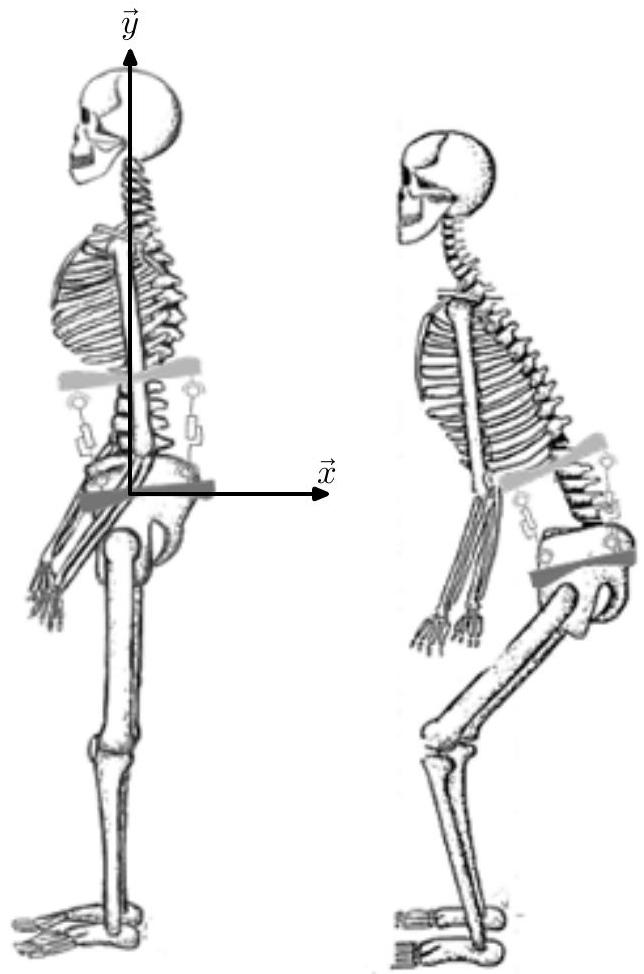
\includegraphics[width=\textwidth]{2025_09_16_5f2d7643f7e649c6833dg-05}
%\captionsetup{labelformat=empty}
%\caption{Figure 6 Mouvement de flexion et implantation de l'exosquelette}
%\end{center}
%\end{figure}


\begin{figure}[!h]
\centering
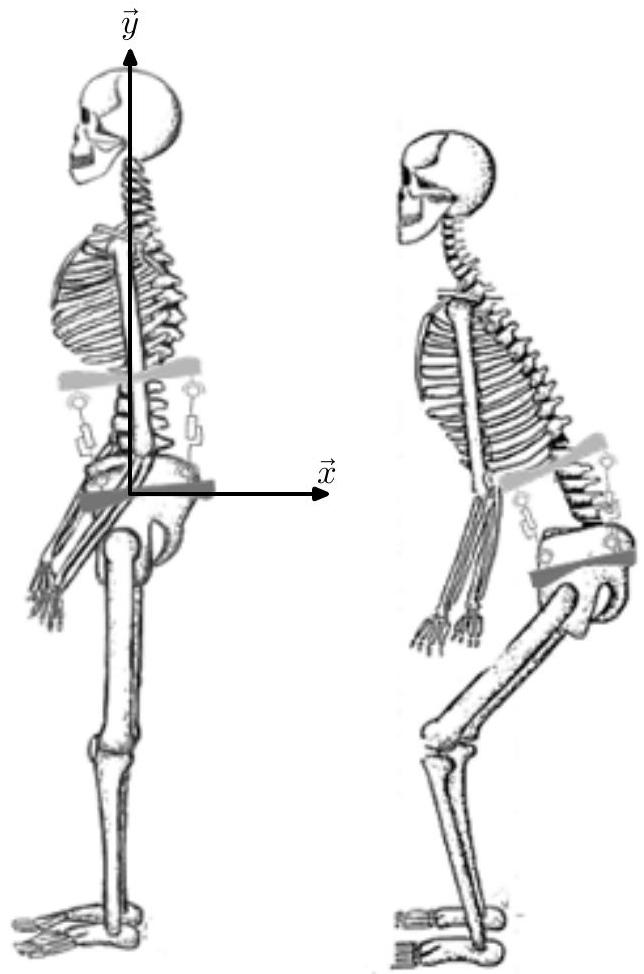
\includegraphics[width=.4\textwidth]{2025_09_16_5f2d7643f7e649c6833dg-05}
\caption{\label{ccs_mp_2023_fig_06}  Mouvement de flexion et implantation de l'exosquelette}
\end{figure}



%\begin{figure}[h]
%\begin{center}
%  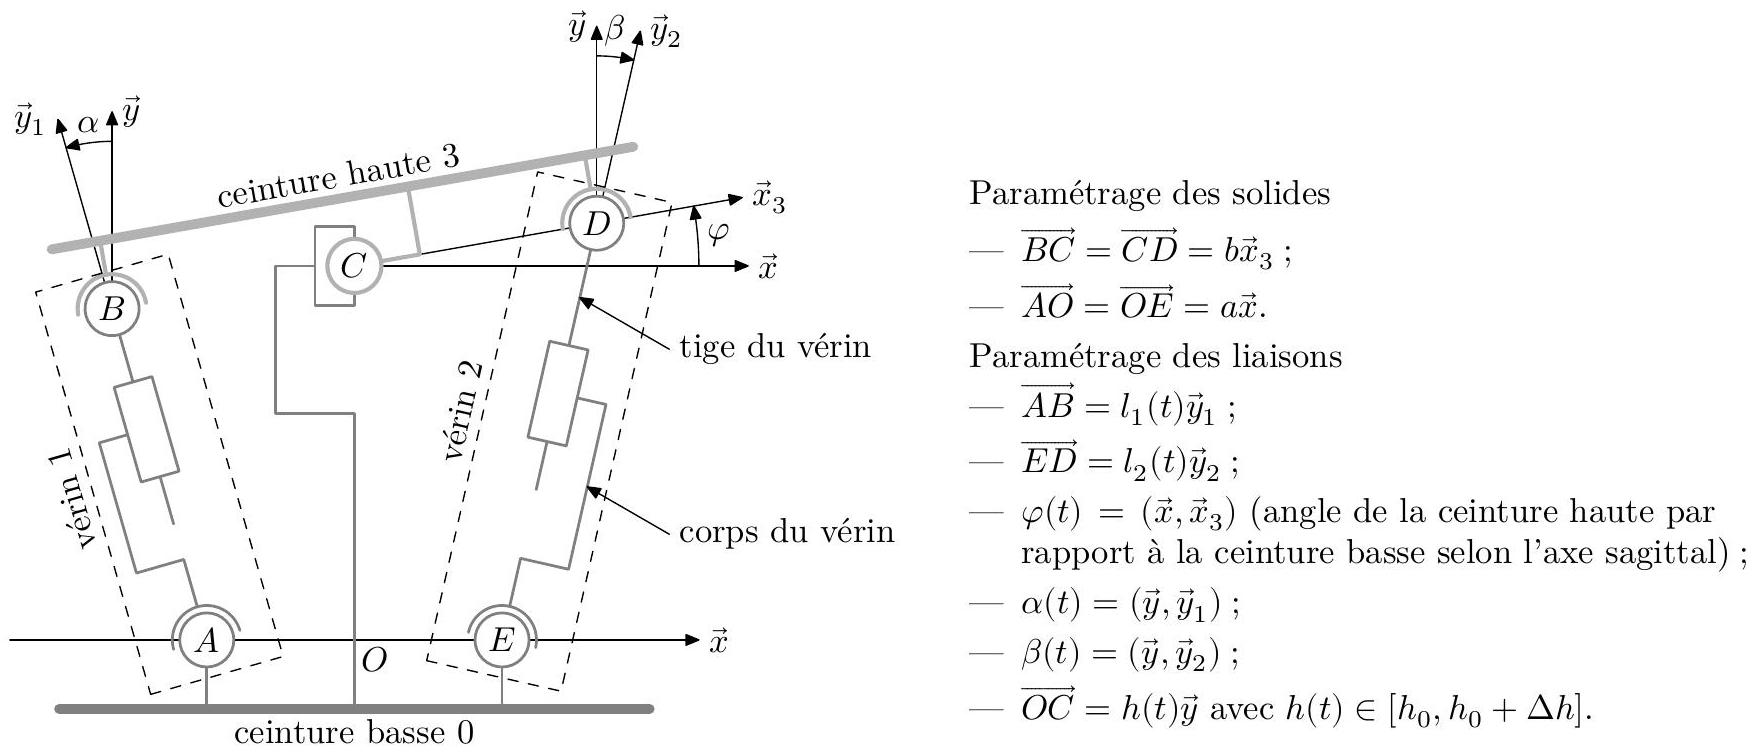
\includegraphics[width=\textwidth]{2025_09_16_5f2d7643f7e649c6833dg-05(1)}
%\captionsetup{labelformat=empty}
%\caption{Figure 7 Paramétrage cinématique}
%\end{center}
%\end{figure}


\begin{figure}[!h]
\centering
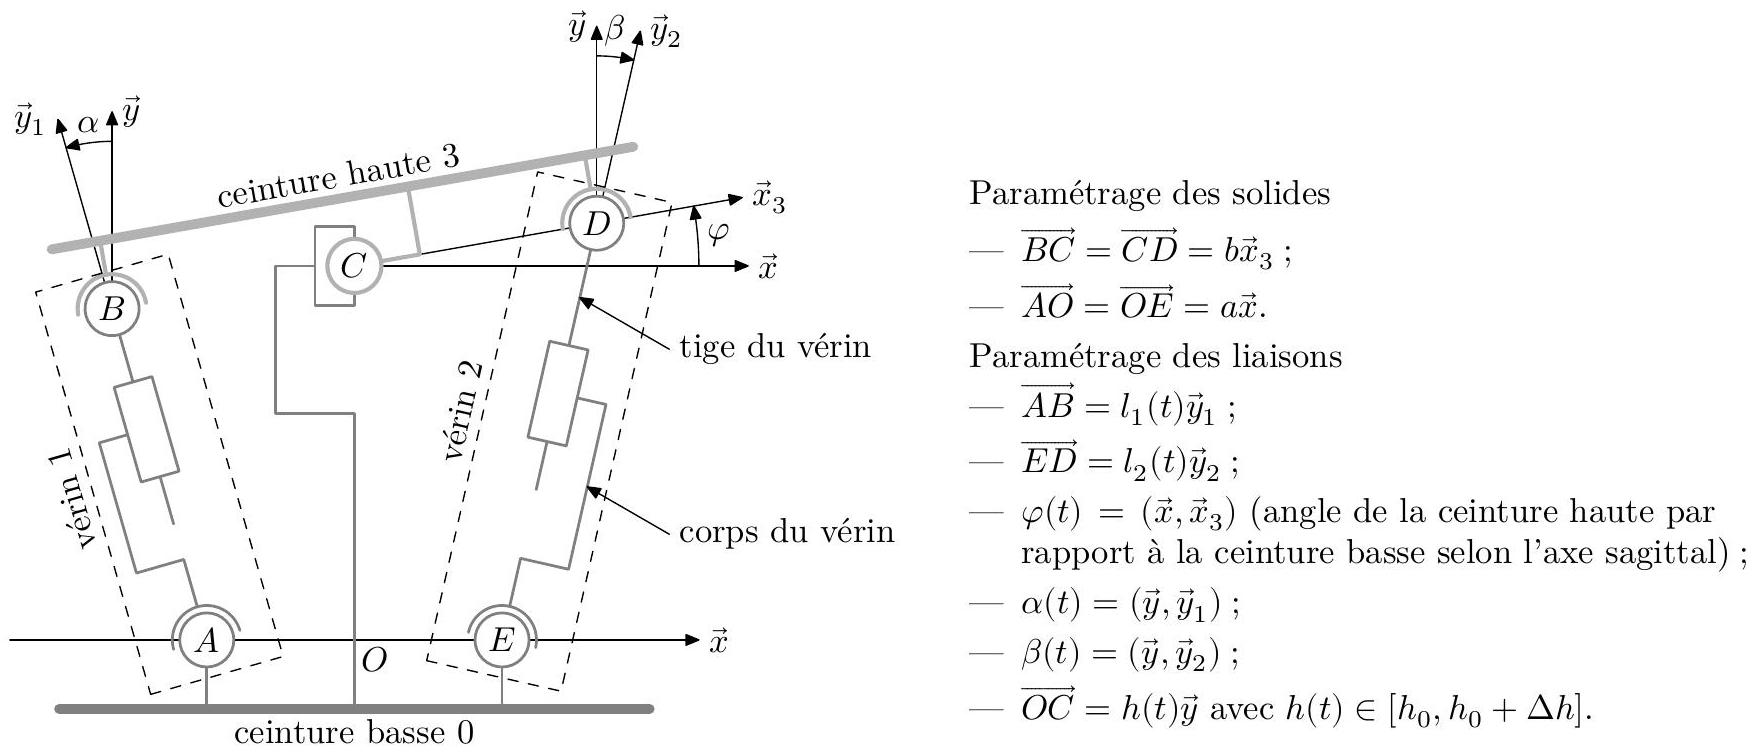
\includegraphics[width=\textwidth]{2025_09_16_5f2d7643f7e649c6833dg-05(1)}
\caption{\label{ccs_mp_2023_fig_07} Paramétrage cinématique }
\end{figure}




Le protocole de mise en précontrainte et d'utilisation de l'exosquelette est le suivant:

\begin{enumerate}
  \item à $t=0$, mise en place de l'ensemble en ajustant sur le corps de l'usager les deux ceintures basse et haute $\left(h_{0}=h(0)\right)$;
  \item pour $t \in[0, T]$, mise en précontrainte $\left(h(T)=h_{0}+\Delta h\right)$;
  \item pour $t>T$, mouvement libre (dans notre étude, $\varphi(t)$ est limité de $0^{\circ}$ à $20^{\circ}$ selon l'axe sagittal).
\end{enumerate}

On définit la course d'un actionneur linéaire comme étant la distance que peut parcourir la tige par rapport au corps entre ses positions extrêmes.\\
\fi

%Q 4. 
\question{\label{ccs_mp_2023_q_04}
Le point $C$ restant sur l'axe $\axe{O}{y}$, déterminer la course du vérin 2 à partir du protocole défini précédemment pour les valeurs $a=100 \mathrm{~mm}, b=150 \mathrm{~mm}, h_{0}=100 \mathrm{~mm}$ et $\Delta h=50 \mathrm{~mm}$.}
\ifprof
\begin{corrige}
En $t=0$, on a $\varphi = 0$ et donc 
$l_2^2(t) = \left(b -a  \right)^2  +  h(t)^2  $
$\Leftrightarrow l_2^2(t) = \left(b -a  \right)^2  +  h(t)^2  $.
On a donc $l_2(0) = \SI{112}{mm}$.

Le vérin sera davantage déployé si l'exosquelette est incliné en plus d'être décalé sur $h$.
 En $t=T$, $\varphi = 20\degres$ et $h = 150$ on a 
 $l_2(0) = \SI{205}{mm}$.
 
 Au final la course du vérin est de \SI{93}{mm}.

\end{corrige}
\else
\fi

\ifprof
\else

Une étude équivalente montre que la course du vérin 2 est supérieure à celle du vérin 1.

La course obtenue permet donc de dimensionner géométriquement les actionneurs en fonction des positions des points d'accroche sur les ceintures haute et basse. On peut ainsi définir la valeur de contrôle à mettre en place sur le banc d'essai. Cette valeur est vérifiée pour chaque actionneur fabriqué.\\
L'exigence sur la liberté de mouvement angulaire étant vérifiée, la suite de l'étude a pour but de caractériser la dynamique et la commande d'un des quatre actionneurs ce qui nécessite l'élaboration d'un modèle de connaissance. La validation sera faite à partir des résultats de la force de traction mesurée sur le banc d'essai.
\fi

%%%% DEBUT AJOUT %%%
\subsection{Analyse de la structure cinématique de l'exosquelette} % Ajout XP

\ifprof
\else

On note $C_1$ le cors du vérin 1, $T_1$ la tige du vérin 1, $C_2$ le cors du vérin 2, $T_2$ la tige du vérin 2.
La ceinture basse est notée 0 et la ceinture haute est notée 3. 

On donne sur la figure suivante le paramétrage des angles de la rotule de centre $A$.  Elle est donc paramétrée par les angles $\psi_1$, $\theta_1$ et $\alpha_1$.

Par ailleurs, on note $\vecto{3}{T_1}$ le vecteur instantanné de rotation de 3 par rapport à $T_1$.  $\vecto{3}{T_1} = \dot{\psi_2} \vx{1}+\dot{\theta_2} \vy{1}+\dot{\alpha_2} \vz{1}$
\begin{center}
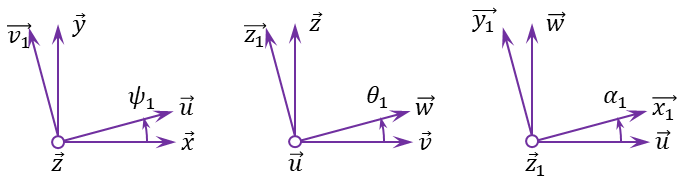
\includegraphics[width=.8\textwidth]{2023_mp_ccs_fig_02.png}
\end{center}
 \fi
 
 
\question{Tracer le graphe des liaisons associé au modèle d'exosquelette proposé figure \ref{ccs_mp_2023_fig_07}.}
\ifprof
\begin{corrige}
\begin{center}
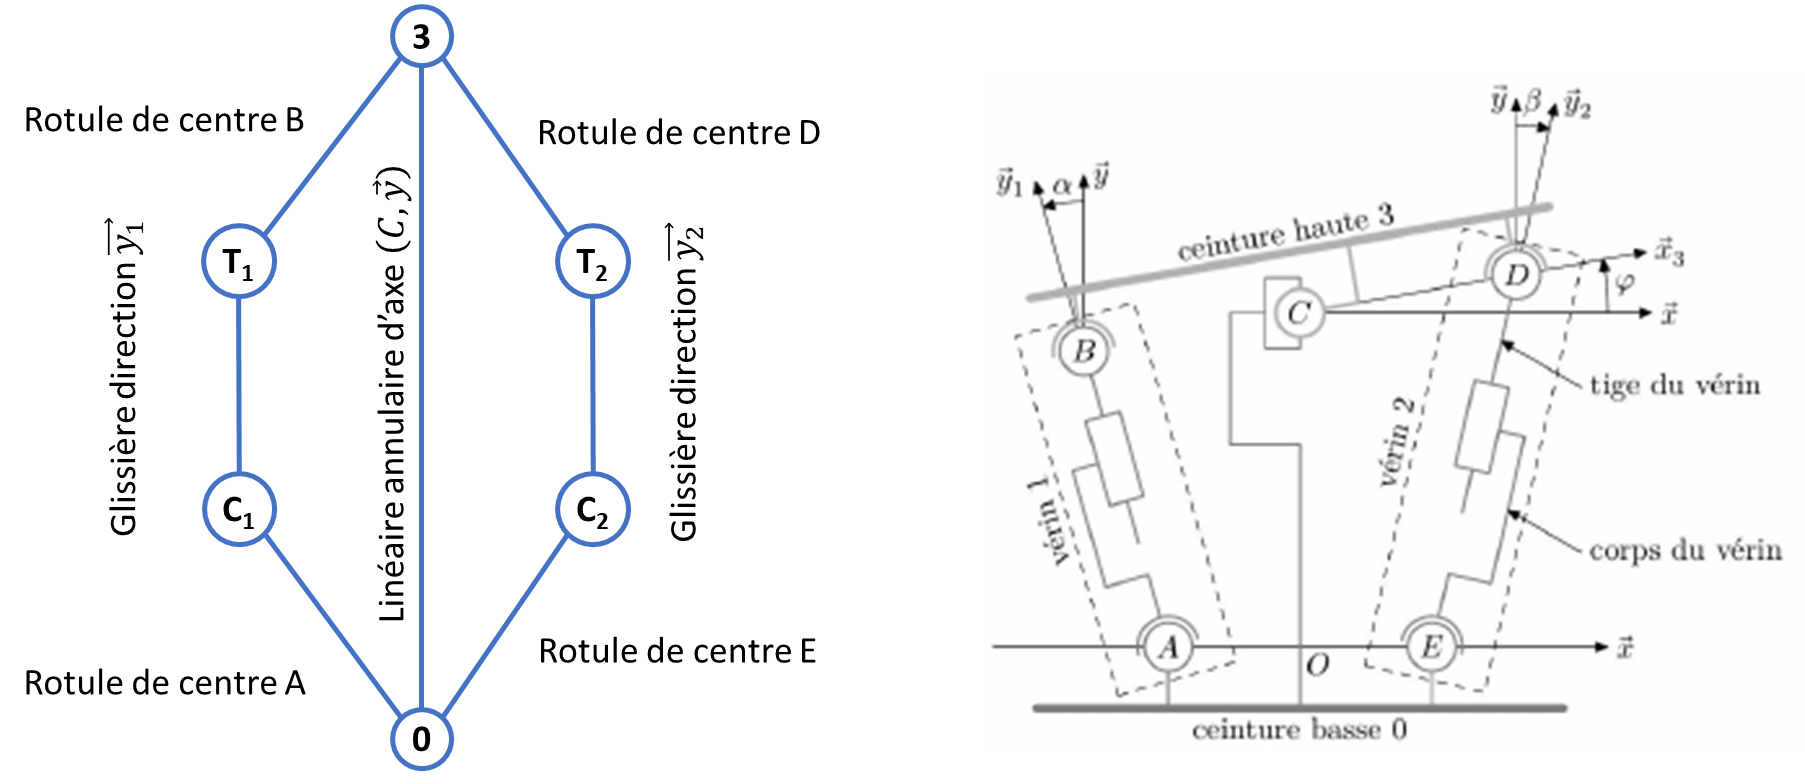
\includegraphics[width=.8\textwidth]{2023_mp_ccs_corr_01}
\end{center}
\end{corrige}
\else
\fi

\question{\textbf{Sans calcul}, proposer une méthode permettant de déterminer la liaison équivalente entre la ceinture basse \textbf{0} et la ceinture haute \textbf{3}.}
\ifprof
\begin{corrige}
\begin{itemize}
\item Sur la branche $0 - C_1 - T_1 - 3$, les liaisons sont en série. On va sommer les torseurs cinématiques pour déterminer la liaison équivalente.
\item Sur la branche $0 - C_2 - T_2 - 3$, les liaisons sont en série. On va sommer les torseurs cinématiques pour déterminer la liaison équivalente.
\item Les pièces 0 et 3 sont alors reliées par 3 liaisons en parallèle. On somme donc les torseurs statiques.. 
\end{itemize}

On peut intuiter que les liaisons vérins entre deux rotules formeront des liaisons libres (6 degrés de libertés). La liaison équivalente sera donc la liaison annulaire d'axe $\axe{C}{y}$.
\end{corrige}
\else
\fi



\question{Exprimer le torseur cinématique de la liaison équivalente entre le solide 3 et le solide 0 en passant par le vérin 1 au point $B$. Exprimer ensuite le torseur de la liaison des actions mécaniques.}
\ifprof
\begin{corrige}
On a $\torseurcin{V}{3}{0} = \torseurcin{V}{3}{T_1} + \torseurcin{V}{T_1}{C_1} + \torseurcin{V}{C_1}{0}$.
 
Seul $\torseurcin{V}{C_1}{0}$ est à déplacer au point $B$. 

On a $\vectv{B}{C_1}{0} = \vectv{A}{C_1}{0} + \vect{BA}\wedge \vecto{C_1}{0}$ 
$ = -\ell_1\vect{y_1}\wedge \left( \dot{\psi_1} \vect{z}+\dot{\theta_1} \vect{u}+\dot{\alpha_1} \vz{1}\right)$ 

$ = -\ell_1 \left( \dot{\psi_1} \vect{y_1}\wedge \vect{z}+\dot{\theta_1}\vect{y_1}\wedge \vect{u}+\dot{\alpha_1} \vect{y_1}\wedge\vz{1}\right)$ 
$ = -\ell_1 \left( \dot{\psi_1} \vect{y_1}\wedge \left( \cos\theta_1\vz{1}+\sin\theta_1\vect{w} \right)-\dot{\theta_1}\cos\alpha_1  \vect{z_1}+\dot{\alpha_1} \vect{x_1}\right)$ 

$ = -\ell_1 \left( \dot{\psi_1} \left( \cos\theta_1 \vect{x_1} - \sin\theta_1 \sin\alpha_1\vect{z_1} \right)-\dot{\theta_1}\cos\alpha_1  \vect{z_1}+\dot{\alpha_1} \vect{x_1}\right)$ 
$ = u_1 \vect{x_1}+v_1 \vect{y_1}+w_1 \vect{z_1}$.


Au final, 
$\torseurcin{V}{3}{0} = 
\torseurl{\dot{\psi_2} \vx{1}+\dot{\theta_2} \vy{1}+\dot{\alpha_2} \vz{1} + \dot{\psi_1} \vect{z}+\dot{\theta_1} \vect{u}+\dot{\alpha_1} \vz{1}}{u_1 \vect{x_1}+v_1 \vect{y_1}+\dot{\ell_1} \vect{y_1}+w_1 \vect{z_1}}{B}
$

Il s'agit d'une liaison à 6 degrés de libertés (3 rotations et 3 translation). Il s'agit d'une liaison libre. 


Le torseur statique associé est le torseur nul $\torseurstat{T}{3}{0} = \left\{0 \right\}$.
\end{corrige}
\else
\fi

\question{Déterminer la liaison équivalente entre le solide 3 et le solide 0. En déduire le nombre de mobilités utiles du modèle.}
\ifprof
\begin{corrige}
Pour trouver la lisaison équivalente de 3 par rapport à 0, on réalise la somme des 3 torseurs statiques, dont deux sont nuls. 

Il ne reste que la liaison linéaire annulaire initiale.

La liaison à 4 degrés de liberté, il y a donc 4 mobilités utiles. 
\end{corrige}
\else
\fi


\question{Déterminer méthodiquement le degré d'hyperstisme du modèle proposé figure \ref{ccs_mp_2023_fig_07}.}
\ifprof
\begin{corrige}
En utilisant une méthode cinématique, on a : 
\begin{itemize}
\item $m =4 + 2 =6$ : il y a deux vérins birotulés qui ont chacun une rotation propre autour de leur axe. 
\item $I_c = 4 \times 3 + 2 \times 1 + 1\times 4 = 18$ : 4 rotules à 4 DDL, 2 glissière à 1 DDL et 1 LA  à 4 DDL. 
\item $E_C = 2 \times \gamma =12$ équations.
\end{itemize}
Au final, 
$h=m-I_C+E_C = 6  - 18  +12 = 0$. Le système est isosatique.
\end{corrige}
\else
\fi



